\documentclass{article}

\usepackage{fullpage}
\usepackage{amsmath}
\usepackage{amsthm}
\usepackage{graphics}
\usepackage{graphicx}

\newtheorem{theorem}{Theorem}

\author{Olivier Beaumont, Lionel Eyraud-Dubois, Erik Saule}

\title{Fun with recursivity and parallel graph construction}

\begin{document}

\maketitle

\section{Introduction}

The idea is to investigate the general problem of algorithm that have
many versions, some being more parallel than other. At different
stages of the algortihm one may opt to pick a different algorithm to
match teh amount of parallelism available. Though increasing the
parallelism may cost additional work, so doing that smartly is
important. So there is a tradeoff in these problems between work and
critical path. The overall problem in general is how to find these
good configurations.

We look here at some recursive problems where we can certainly derive
the optimal configuration of the algorithm

\section{Multiplying Large Integers}

With $I_1 = aM + b$ and $I_2 = cM + d$ with $a,b,c,d < M$. Assume that
$I_1, I-2$ are of similar length which is $2^k$ words. $M$ is the
basis that maps to $2^{k-1}$ words.

\subsection{Variants}

\subsubsection{Naive}

The naive algorithm taught in elementary school is to compute:

\begin{align}
  I_1 * I_2 & = & a*c M^2 + (a * d + b * c ) M + b*d \\
            & = & (a*c)_{u} M^3 + ((a*c)_{l} + (a * d + b * c )_{u}) M^2 + ( (a * d + b * c )_{l} + (b*d)_{u} ) M + (b*d)_{l}
\end{align}

where the $x_u$ stands for the MSBs of $x$ and $x_l$ stand for the
LSBs of $x$. Indeed when multiplying $a*c$ (for instance), the result
can be almost as large as $M^2$ and therefore can are typically split
in two halves. (Note that there is a carry that bit that is ignored
here.)

\subsubsection{Karatsuba}

%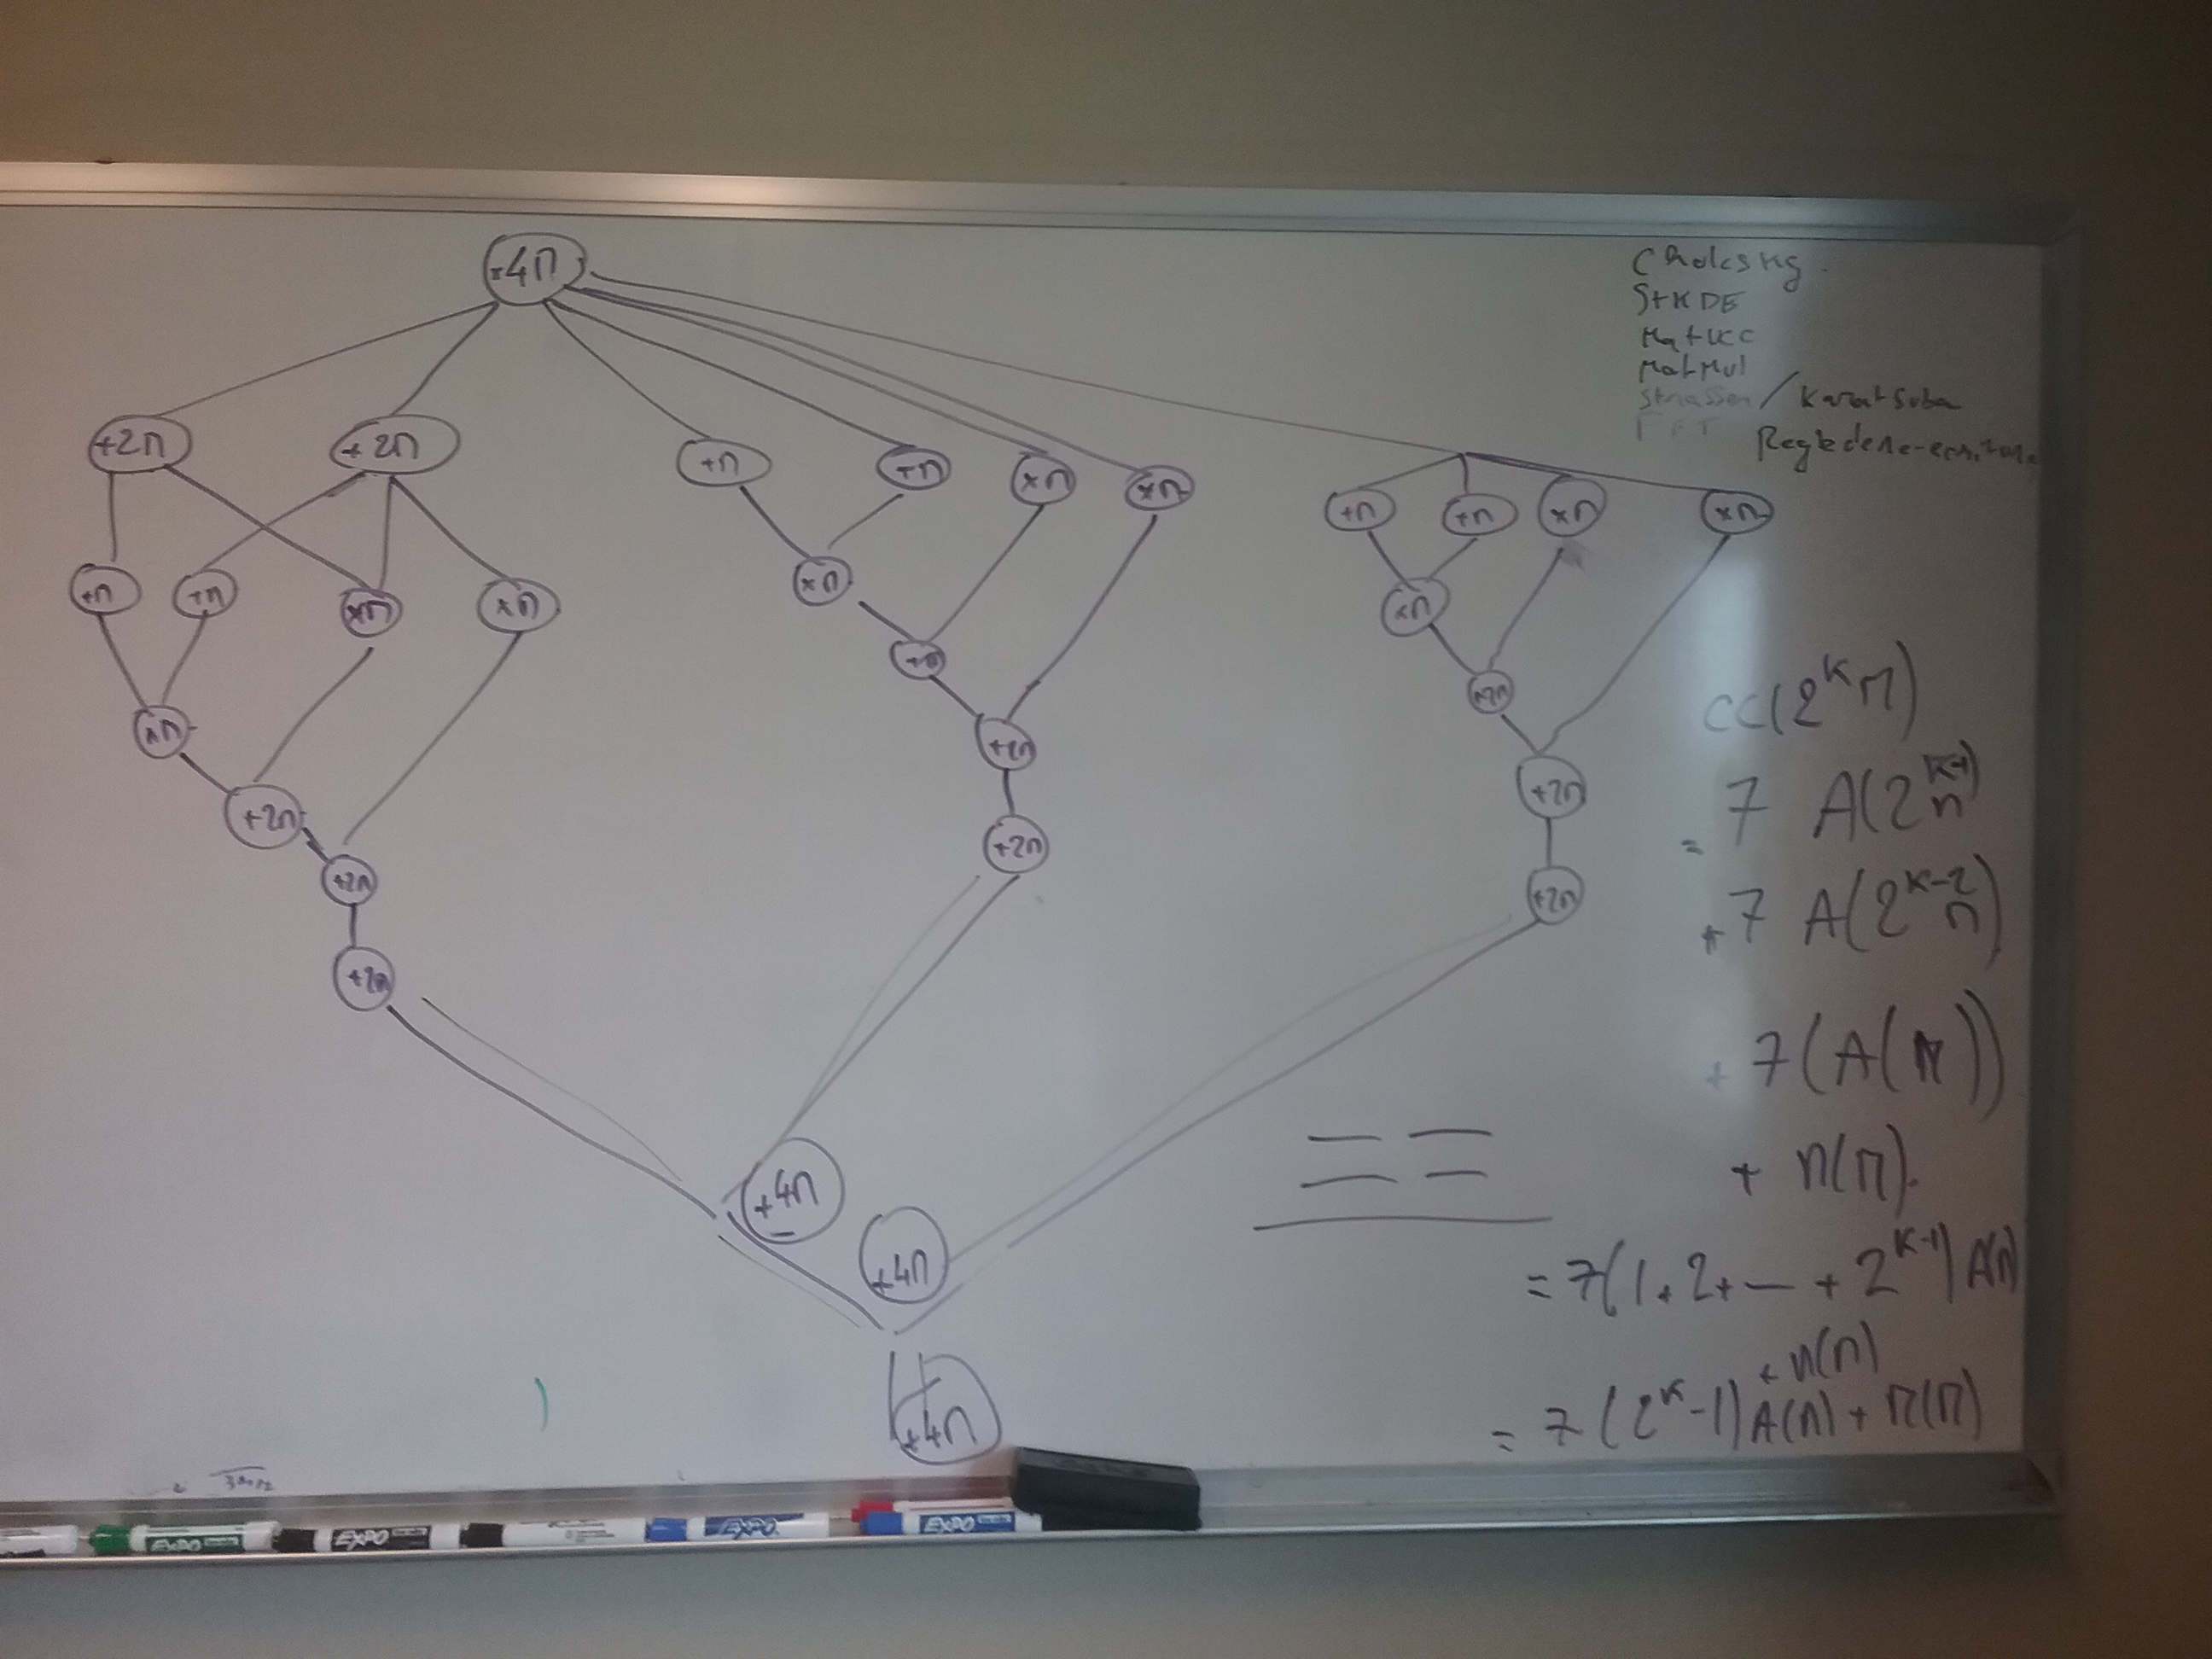
\includegraphics[width=.5\linewidth]{../../notes/20180608_120848.jpg}

Actually in Karatsuba, the critical path is mostly composed of add
tasks. Add tasks can be trivially be made parallel by keeping their
work constant but decreasing the critical path up to $add(1)$. This
makes Karatsuba the algorithm with lowest work and small critical path.

\section{MergeSort}

\subsection{Variants}

\subsubsection{With Sequential Merge}

With sequential merge, we have an in-tree of merges with the root
being of $Merge(n)$, one level down being 2 $Merge(n/2)$, etc.

This leads to $Merge^W(n) = n$ and $Merge^{CP}(n)=n$. $MergeSort^W(n)
= n \log n$ and $MergeSort^{CP}(n) = 2n$.

\subsubsection{With Parallel Merge}

Merge can be made parallel. When merging two arrays of size $n/2$. Cut
the first one in half and find the corresponding cut location in the
second array (using a binary search). To get good load balancem, one
needs to also cut the second array and find the corresponding location
in the first array, leading to 3 chunks that need to be cut.

One can assume that a single cut is enough for analysis purposes,
thought the more complex algorithm is necessary to reach the correct
bounds.

One can generalize that cut by having $P$ cuts, and performing P
binary searches on each side, there is a need to reconcile the cuts
position which cost a merge of size $2P$ (assumed sequential). This leads to $Merge^W(n,P) =
n + 2 P \log n + 2P$, the $n$ term is for all the merges, the $2P \log
n$ are for the binary search and the $2P$ is for the merge of size
$2P$. And $Merge^{CP}(n,P) = n/P + \log n + 2P$, the $n/P$ term
is for the final merge, the $\log n$ comes from the parallel binary
searches, and the $2P$ comes from the merge of size $2P$ in parallel.

Since obtaining more parallelism is a costly operation in term of
work, for ParallelMergeSort, the optimal solution is clearly to have
$P$ tasks for level 0, $P/2$ tasks for each merge at depth 1,
$P/4$ tasks for each merge at depth 2, ... Defaulting to sequential
merges at depth $\log P$

For this parallel merge sort, the work becomes
$ParallelMergeSort^W(n) = n \log n + 2 P \sum_{i=0}^{\log P - 1} \log n/2^i + 1$
since the term in $n$ does not change
from merge sort and the splitting overhead is of $2P (\log n/2^i + 1)$ at
level $i$. So
\begin{align}
  ParallelMergeSort^W(n) & = & n \log n + 2 P \sum_{i=0}^{\log P - 1}( \log n/2^i + 1  )\\
  & = &n \log n + 2 P \left (\log P (\log n +1)- \sum_{i=0}^{\log P - 1} \log 2^i  \right )  \\
  & = &n \log n + 2 P \left (\log P (\log n +1)- \sum_{i=0}^{\log P - 1} i \right )  \\
  & = &n \log n + 2 P \left ( \log P (\log n +1)- \frac{(\log P - 1)(\log P)}{2}   \right) \\
  & = &n \log n + 2 P \log P \left (  \log n + 1 - \frac{\log P - 1}{2}   \right)  
\end{align}

In the critical path, there is a term in $2 n/P$ which comes from the
low sequentil merges Merges and a $Merge^{CP}(n/2^i,P/2^i)$ for each
parallel merge on the CP.
\begin{align}
  ParallelMergeSort^{CP}(n) & = & 2n/P + \sum_{i=0}^{\log P-1} Merge^{CP}(n/2^i,P/2^i) \\
  & = & 2n/P + \sum_{i=0}^{\log P-1} \left ( (n/2^i)/(P/2^i) + \log (n/2^i) + 2P/2^i \right )\\
  & = & 2n/P + \frac{n}{P} \log P  + \log P \log n - \frac{(\log P - 1)(\log P)}{2}  + 4P \\
  & = & 2n/P + 4P + \log P \left ( \frac{n}{P}   +  \log n - \frac{\log P - 1}{2}  \right )
\end{align}

So we have an algorithm (Merge Sort) where part of the graph has
limited parallelism and where adding parallelism can make sense. But
adding too much parallelism is harmful because of the additional work
to be done.

Note that we can predict the shape of the gantt chart pretty easily.

\section{QuickSort}

Note in QS that we can assume that partition always splits in the
middle, since it is probabilistically equivalent to that.

\subsection{With Sequential Partition}

With sequential partition, we have an out-tree of partition with the
root being of $partition(n)$, one level down being 2 $partition(n/2)$,
etc.

This leads to $partition^W(n) = n$ and
$partition^{CP}(n)=n$. $QuickSort^W(n) = n \log n$ and
$QuickSort^{CP}(n) = 2n$.

\subsection{With Parallel Partition}

Partition in parallel is done with a fixed split in $P$ parts. Each
part takes a piece of the array and counts how many entries are less
than, more than the pivot. Then a prefix sum is computed on the number
of less than and more than entries than the pivot so that each piece
knows where to write. Finally, each part is individually written. This
makes

$$partition^W(n, P) = 2 n + 2 PrefixSum^W(P)$$

$$partition^{CP}(n, P) = 2 n/P + 2 PrefixSum^CP(P)$$

The first partition on $n$ elements will be made with a parallelism of
$P$ at level 0, the 2 partition of size $n/2$ at level 1 will be made with a parallelism of $P/2$ each, ...




\end{document}
